%%
%% This is file `sample-manuscript.tex',
%% generated with the docstrip utility.
%%
%% The original source files were:
%%
%% samples.dtx  (with options: `manuscript')
%% 
%% IMPORTANT NOTICE:
%% 
%% For the copyright see the source file.
%% 
%% Any modified versions of this file must be renamed
%% with new filenames distinct from sample-manuscript.tex.
%% 
%% For distribution of the original source see the terms
%% for copying and modification in the file samples.dtx.
%% 
%% This generated file may be distributed as long as the
%% original source files, as listed above, are part of the
%% same distribution. (The sources need not necessarily be
%% in the same archive or directory.)
%%
%% Commands for TeXCount
%TC:macro \cite [option:text,text]
%TC:macro \citep [option:text,text]
%TC:macro \citet [option:text,text]
%TC:envir table 0 1
%TC:envir table* 0 1
%TC:envir tabular [ignore] word
%TC:envir displaymath 0 word
%TC:envir math 0 word
%TC:envir comment 0 0
%%
%%
%% The first command in your LaTeX source must be the \documentclass command.
\documentclass[manuscript,screen,review,sigconf]{acmart}

%%
%% \BibTeX command to typeset BibTeX logo in the docs
\AtBeginDocument{%
  \providecommand\BibTeX{{%
    \normalfont B\kern-0.5em{\scshape i\kern-0.25em b}\kern-0.8em\TeX}}}

%% Rights management information.  This information is sent to you
%% when you complete the rights form.  These commands have SAMPLE
%% values in them; it is your responsibility as an author to replace
%% the commands and values with those provided to you when you
%% complete the rights form.
\setcopyright{acmlicensed}
\copyrightyear{2018}
\acmYear{2018}
\acmDOI{XXXXXXX.XXXXXXX}


%%
%% Submission ID.
%% Use this when submitting an article to a sponsored event. You'll
%% receive a unique submission ID from the organizers
%% of the event, and this ID should be used as the parameter to this command.
%%\acmSubmissionID{123-A56-BU3}

%%
%% For managing citations, it is recommended to use bibliography
%% files in BibTeX format.
%%
%% You can then either use BibTeX with the ACM-Reference-Format style,
%% or BibLaTeX with the acmnumeric or acmauthoryear sytles, that include
%% support for advanced citation of software artefact from the
%% biblatex-software package, also separately available on CTAN.
%%
%% Look at the sample-*-biblatex.tex files for templates showcasing
%% the biblatex styles.
%%

%%
%% The majority of ACM publications use numbered citations and
%% references.  The command \citestyle{authoryear} switches to the
%% "author year" style.
%%
%% If you are preparing content for an event
%% sponsored by ACM SIGGRAPH, you must use the "author year" style of
%% citations and references.
%% Uncommenting
%% the next command will enable that style.
%%\citestyle{acmauthoryear}

%%
%% end of the preamble, start of the body of the document source.
\begin{document}

%%
%% The "title" command has an optional parameter,
%% allowing the author to define a "short title" to be used in page headers.
\title{Can Large Language Models Generated Code For Small-Scale Problems That Is Competitive To Model, Human-Written Code}

%%
%% The "author" command and its associated commands are used to define
%% the authors and their affiliations.
%% Of note is the shared affiliation of the first two authors, and the
%% "authornote" and "authornotemark" commands
%% used to denote shared contribution to the research.
\author{Thomas D. Chambers}
\email{tc262389@falmouth.ac.uk}
\affiliation{%
  \institution{Falmouth University}
  \city{Penryn}
  \state{Cornwall}
  \country{United Kingdom}
  \postcode{TR10 9FE}
}

%%
%% By default, the full list of authors will be used in the page
%% headers. Often, this list is too long, and will overlap
%% other information printed in the page headers. This command allows
%% the author to define a more concise list
%% of authors' names for this purpose.
\renewcommand{\shortauthors}{Trovato and Tobin, et al.}



%%
%% The code below is generated by the tool at http://dl.acm.org/ccs.cfm.
%% Please copy and paste the code instead of the example below.
%%
\begin{CCSXML}

\end{CCSXML}

%\ccsdesc[500]{Do Not Use This Code~Generate the Correct Terms for Your Paper}
%\ccsdesc[300]{Do Not Use This Code~Generate the Correct Terms for Your Paper}
%\ccsdesc{Do Not Use This Code~Generate the Correct Terms for Your Paper}
%\ccsdesc[100]{Do Not Use This Code~Generate the Correct Terms for Your Paper}

%%
%% Keywords. The author(s) should pick words that accurately describe
%% the work being presented. Separate the keywords with commas.
%\keywords{Do, Not, Us, This, Code, Put, the, Correct, Terms, for,
  %Your, Paper}

\received{20 February 2007}
\received[revised]{12 March 2009}
\received[accepted]{5 June 2009}

%%
%% This command processes the author and affiliation and title
%% information and builds the first part of the formatted document.
\maketitle

\section{Introduction}
% What is the study in a few words
This study will be investigating the practicality of using large-language models to generate code. These models take in a human-written prompt to generate an output, hopefully fulfilling the desired task of the prompt. Within the last few years, these models have been used to generate code in many programming languages, straight into a programmer's IDE. With many large tech companies investing in generative models, such as Google and META \cite{Google_AI_2023, Meta_2023}, and bespoke versions of these models being used commercially for code productivity, such as Github's Copilot and Sourcery \cite{GitHub_2021, Sourcery_2023}, their use by programmers is rapidly increasing. Due to the black-box nature of these models, an intimate understanding of how these code snippets are generated is unknown, and there's a risk that poorly written, buggy and insecure code could be used by novice and experienced programmers alike. The need to understand the level of quality of outputs is paramount before these generation tools become widespread in education and industry. The focus of this study will be on Open-AI's GPT models due to their API, success and public prominence.

\section{Understanding Code Generation}
% History of Code Generation
Code generation is not new, being used in many computing processes already, perhaps most well-known is the use in compilers to produce code optimisation and executable machine code. Furthermore, code generation from a human prompt has been discussed for over 50 years. PROW \cite{PROW} was an early code generation tool that could produce Perl code from an input written in predicate calculus. However, as discussed two years later by Manna and Waldinger \cite{Program_Syn}, "programmers might find such a language lacking in readability and conciseness." They went on to predict a future program synthesizer; one that works with the programmer to produce segments of code that can be incorporated into the program. They argue it would be a "more practical system" with greater "power".

% Public release of ChatGPT has blown up popularity
Fifty years later in 2022, the public release of ChatGPT\cite{ChatRel}, caused the public awareness of LLM  to skyrocket. Generation models have been used for years to write essays, generate art and synthesise an actor's voice, the implications of such have sent shock waves through educational and business environments \cite{GPTBusinessImpact, GPTEducationImpact, ethicalImpact, LaborMarketImpact}, but more recently the use of generation has become more relevant in a programmer's workflow.

% Generated code evolution up to codex then CoPilot
\subsection{The Background of LLM}
% How do LLM work roughly (not super important for this paper but it does need to be in here. Almost all papers leave it out as assumed knowledge so just a quick overview is sufficient)
The rising popularity of LLM generation is mainly due to their apparent success at task completion, giving them the appearance of being \textit{intelligent}. Large language models are neural networks trained to predict the next token in a sequence.
\[P(Token_n|Token_1,Token_2,...,Token_{n-1})\]
GPT stands for \textbf{G}enerative \textbf{P}re-trained \textbf{T}ransformer. The generation means that it can predict the next token, pre-trained means that the model has received a large amount of data and has had its bias adjusted and a transformer is an encoder-decoder network that adds \textit{self-attention}. Self-attention results in significant performance increases in accurate prediction. LLM that have been pre-trained can be further \textit{fine-tuned} to improve performance at specific predictions.

%%% Discussion about the studies performance of LLM tools already in use %%%

In 2021 OpenAI released their fine-tuned model GPT-3 codex, trained on 54 million public software repositories hosted on GitHub\cite{CodexRelPaper}. Released the same year \cite{GitHub_2021}, Github's CoPilot is a generation model with a heavy reliance on Codex. To test the functional performance of Codex, the team behind OpenAI released the humanEval data set. A public repository to benchmark the performance of generated code. They also implemented the technique \textit{pass@k}. An unbiased calculator to estimate the success of a model given \textit{k} samples. Functional performance is found by the ability to generate code from a prompt that successfully passes given unit tests, failures often due to syntax errors, invoking out-of-scope functions or referencing non-existent variables. Within their data set, Codex had a higher performance than every previous GPT-model, solving 70.2\% of problems with 100 samples. The functional performance of Codex and models alike have been replicated numerously \cite{SysEvaOfLLMofCode, PerformanceParsonProblems, CopilotSuggestionsEval, CoPilotForTeaching}, with Codex being able to outperform students in even CS1 questions and, although performance drop, still compete with students in CS2 questions\cite{Codex_CS1_CS2_Test}. At the higher end of computing problems, the model can recognise algorithms by name and produce efficient solutions for those problems, such as tree or graph searches and modifications.

\subsection{Issues with the Current State of Code Generation}
 Large language models have proven to appear highly performant, however, there are several technical and practical limitations that should be carefully understood.

Firstly, models are not uniform across languages. Nguyen and Nadi \cite{CopilotSuggestionsEval} found that CoPilot functionally performed best when writing in Java and worst in Javascript. Other researchers have written their own fine-tuned model, Poly-Coder, based on the GPT-2 architecture, which outperforms all GPT-based models in the C language \cite{SysEvaOfLLMofCode}. This was argued to possibly be a problem with the dataset and fine-tunning process.

Secondly, the results are not \textit{one-shot}. Codex can respond with very variant accuracy in its solutions, hence why most investigations use several responses, such as with \textit{pass@k} often using 100 samples. This is not the standard programming experience. A student does not submit 100 solutions to be marked by their professor, leading to the comparison being fallacious. An attempt to control this compared students to Codex, except also gave students multiple attempts at solutions, their success frequently increases with each attempt. However, they found that Codex was still competitive with students, even after
 multiple submission\cite{Codex_CS1_CS2_Test}.

Thirdly, responses vary significantly depending on the value of the model temperature. Multiple studies have found that with a higher temperature, models can achieve a higher \textit{pass@k} score at higher samples, despite producing more erroneous code. Across multiple studies, researchers found optimal performance at T0.6, with T0.2 and T0.8 also performing well. Temperature and sample size were found to be proportional, this is likely due to the diversity of code at higher temperatures needing a higher sample rate to score.\cite{stackOVerflowAndTemperature, SysEvaOfLLMofCode, CodexRelPaper}.

Fourthly, there is a significant reason to question whether the success of generated code translates into actual programmer performance, even with their access becoming more streamlined. CoPilot can directly embed into your IDE, finishing off lines or blocks of code for the user. There is also a chat option in VS Code where prompts can be given and code can be directly copied into the user's file. However, when a programmer uses a piece of code, it might be buggy, a sub-optimal solution or poorly written. In a study of 24 participants using Copilot\cite{Expectation_vs_Experience}, they found that even though code generation gave promising results, it did not improve overall programming time or the success rate of those participants using the tool. CoPilot even led to more task failures in the medium and hard category, where programmers might have not understood the generated code or spent longer debugging the code than if they had just written it themselves. However, 23/24 of the participants still found it more useful than Intellisense and the majority "overwhelmingly preferred using Copilot in their programming workflow since Copilot often provided a good starting point to approach the programming task." In this sense, generation acts as a double-edged sword for productivity and learning. On the one hand, it can allow a programmer to instantly generate an often feasible solution to a task, a useful tool. However, in doing so they remove themselves from the task of problem-solving, which often exposes the programmer to online discussion and related topics, advancing their technical skill. Other researchers have discussed this problem, hypothesising that code generation is an efficient tool for seasoned programmers, but can turn into a liability when used by novice programmers who do not fully understand the problem, context and generated solution.\cite{CopilotPairProgrammer}.

\section{Quality Code}
% Importance of code analysis, reference Dijkstra, maybe clean code and Goole/Ibm
Good quality code is vital for creating maintainable software that can last, but still, there is discourse around what good quality code is. In 1969 Dijkstra wrote in a letter, \textit{"A programmer has only done a decent job when his program is flawless and not when his program is functioning properly only most of the time."} He criticized the attitude of programmers of his time, something that he saw as a \textit{"software crisis"}. He saw programmers treating debugging as a necessity, rather than what he believed, an inevitable consequence of poorly written systems. He argued that writing \textit{"intellectually manageable" programs} would reduce the amount of reasoning involved in justifying their proper operation and a reduction in the number of test cases. If done correctly, he claims that \textit{"the correctness can be shown a priori"}, so a need for zero test cases. Dijkstra had laid out a fundamental argument for why quality code is necessary which has been built upon ever since\cite{EWD:EWD288}.

Recognising when code is \textit{"intellectually manageable"} is harder said than done. Greg Michaelson wrote that \textit{"Programming style is notoriously difficult to characterise"} and that imperative languages have been the \textit{"source of endless theological disputes"}, such as the use of GOTOS, the use of recursion over iteration or the number of parameters a sub-program should have\cite{Automatic_analysis}. While for the most part, experts agree on the abandonment of goto's in structured programming \cite{gotoConsideredHarmful, KnuthGoTo}, the rest are still up for debate.

Clearly, the quality of generated code is vital if the produced code is ever expected to be used in a practical sense. However, the common mantra, \textit{garbage in, garbage out} is just as true now \cite{simmons2023garbage}, the quality of written code largely depends on the quality of the code within the data set. Unfortunately,  the fine details of the data sets used for available LLM are kept private, \cite{SysEvaOfLLMofCode}, so to assess the quality of code, we can use code metrics as an attempt to score the outputted code.


\subsection{Code Analysis}
% Write about different code metrics and how they've been used to measure student work
Pre-1980, software metrics generally worked as a regression model between two variables, conceptually simple, mostly relying on resources and quality. However, during the mid-late 70s, software metrics saw a new direction with Halstead and McCabe\cite{FENTON1999149}. They extracted information from the code design rather than just the static code.

Halstead developed a set of formulas that, when given a code input, would produce a series of scores based on the number of unique and total amount of operands and operators used\cite{Halstead}. The definition of Operands and Operators has slightly different meanings depending on the implementation, but generally, operators are all normal operators, keywords and brackets of all kinds ( (), [], {} ). Operands are variables, methods or function declarations and constants such as Boolean values and strings. Halstead metrics produce useful scores of the complexity of code, such as an estimate of the time to program and the potential for bugs. Although Halstead metrics are not free from critique, various definitions can cause trouble when comparing scores, the use of magic numbers (18 appearing in the Time formula) appears to be arbitrary and it can be argued that the use of operands and operators is too simplistic for modern programming.

Other code metrics take different approaches to Halstead to achieve the same goal of scoring code. The \textit{Flesch-Kincaid readability test} \cite{FleschReading} is a method to score the readability of human written language, based on the number of \textit{syllables per words} and \textit{words per sentence}, similar to how Halstead used operators and operands. Kurt Starsinic developed a module, \textit{Fathom.pm}, to apply the Fleshc-Kincaid test to Perl code, producing a score based on the number of \textit{{}tokens per expression}, \textit{expressions per statement} and \textit{statements per subroutine}. \cite{Starsinic_1998}.
\\ \\
Code Complexity =\\
  ((average expression length in tokens) * 0.55)\\
+ ((average statement length in expressions) * 0.28)\\
+ ((average subroutine length in statements) * 0.08)\\
\\
The formula would produce a score from 1 - 7, where 5 is "Trival" and 7 is "Very Hairy".  However, he did not provide any justification for the weights used in the formula except that they were fined-tuned through trial and error.
Börstler, Caspersen and Nordström would later produce a similar metric method to Starsinic, while also using the FLesch-Kincaid test. They introduced the Software Readability Ease Score (SRES) by treating the "lexemes of a programming language as syllables, its statements as words, and its units of abstraction as sentences" \cite{borstler2007beauty}. They argued that this type of static code analysis was a clear indicator of how readable, and thus maintainable the code was. However, to quote Dijkstra, other factors affect the "\textit{goodness}" of code, such as control flow.

In 1976, McCabe proposed a technique called \textit{Cyclomatic complexity} for scoring the control flow a program takes \cite{A_Complexity_Measure}. This was an attempt to "\textit{provide a quantitative basis for modularization}" as a way to identify in advance modules which will be difficult to maintain. McCabe provides the definition
"\textbf{Definition 1:} \textit{The cyclomatic number V(G) of a graph G
with n vertices, e edges, and p connected components is}

\[v(G)=e- n+p\]
\\
Cyclomatic complexity can be viewed as building up graphs from smaller components, examples of which McCabe included.
\begin{figure}[h]
    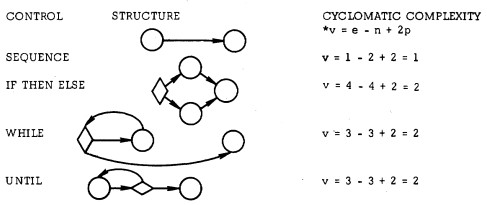
\includegraphics[width=8cm]{controlFlowDia.jpg}
    \caption{Generated Control Structure Graphs}
    \label{fig:CC Graphs}
    \centering
\end{figure}

However, Cyclomatic complexity does not tell the full picture of code, especially since it does not consider else, do \& try, object creation and method calls. Furthermore, there are different interpretations of the method, with some researchers testing complexity at only a module level, while others at a program level, summing up the scores of individual modules. This inconsistency disrupts the comparison of results.\cite{McCabeCritique, NoviceCodeWriting}.  While none of these metrics are perfect estimates of complexity, they allow for fast, accurate judgment of code. Halstead and McCabe developed their metrics during an era of batch programming where systems were significantly smaller today. While they may be ill-suited for large, industrial software, this makes them the perfect solution to measuring smaller, generated code pieces which inherently lack the complexity in which these metrics can not accurately judge\cite{metricCritique}.

% Talk about how there is a gap in the research when it comes to the analysis of generated code
To accurately ascertain a meaningful judgement of code quality, several measurements must be taken that account for the complexity of each line \textit{and} the path the code can take throughout the program. This approach of using code metrics to judge LLM generation is sparse in the current field of research\cite{CopilotPairProgrammer, CopilotSuggestionsEval}, with researchers focusing on functional performance. The practicality of code generation relies in large part on the maintainability of the code, not just its functional performance, and is in need of better understanding.

\section{Aim of Research}
% Research Question & Hypothesis
\textbf{RQ:} Can large language models generate code for small-scale problems that compete with model, human-written answers.\\
\textbf{Hypothesis:} Large language model can generate code for small-scale coding problems that produces equal or better scoring in given code metrics when compared to model, human answers.

\section{Artefact}
% Rich Description

% Development Method (System Lifecycle)

% Quality Assurance

\section{Research Methods}
% Philosophical Position

% Research Method (Sampling/Measurements/Experimental Design)

% Ethical Considerations (Joe as a collaborator, no participants)

\section{Hypothesis Testing}
% Stats and R n shit

\section{Issues and Implications of the Study}
% Students could become too reliant
% Students could pass of generated code as their own in the same way humanity students can with ChatGPT. This has far-reaching implications.
%



%% The acknowledgements section is defined using the "acks" environment
%% (and NOT an unnumbered section). This ensures the proper
%% identification of the section in the article metadata, and the
%% consistent spelling of the heading.
\begin{acks}
Thank you Joseph Walton-Rivers for providing the model answers
\end{acks}

%%
%% The next two lines define the bibliography style to be used, and
%% the bibliography file.
\bibliographystyle{ACM-Reference-Format}
\bibliography{base}


\end{document}
\endinput
%%
%% End of file `sample-manuscript.tex'.
